\section{Program Generation}
\label{sec:related-work-generation}

The generation of artificial programs is a broad field with a wide range of applications. This section categorises the literature the use cases that are relevant to this thesis: program generation for performance characterisation, and program generation for compiler validation.

\subsection{Performance Characterisation}
\label{subsec:training-with-synthetic-benchmarks}

Benchmarks do not cover the whole space / are not representative:

% Ryoo, J. H., Quirem, S. J., Lebeane, M., Panda, R., Song, S., & John, L. K. (2015). GPGPU Benchmark Suites: How Well Do They Sample the Performance Spectrum? ICPP.
\todo[inline]{Evaluating GPGPU benchmarks. There are parts of the space left untested~\cite{Ryoo2015}.}

% Goswami, N., Shankar, R., Joshi, M., & Li, T. (2010). Exploring GPGPU workloads: Characterization methodology, analysis and microarchitecture evaluation implications. In IISWC. https://doi.org/10.1109/IISWC.2010.5649549
\todo[inline]{Evaluation of many benchmark suites. \emph{Similarity Score}, \emph{Scan of Large Arrays}, and \emph{Parallel Reduction} workloads show significantly different behavior due to their large number of diverse kernels, whereas the rest of the workloads provide similar characteristics~\cite{Goswami2010}.}

% Xiong, W., Yu, Z., Bei, Z., Zhao, J., Zhang, F., Zou, Y., … Xu, C. (2013). A Characterization of Big Data Benchmarks. In Big Data. IEEE. https://doi.org/10.1109/BigData.2013.6691707
\todo[inline]{Workload behaviour is highly input dependent, the benchmarks created for academic research cannot represent the cases of real world applications~\cite{Xiong2013}.}

% Ferdman, M., Adileh, A., Kocberber, O., Volos, S., Alisafaee, M., Jevdjic, D., … Falsafi, B. (2012). Clearing the Clouds: A Study of Emerging Scale-out Workloads on Modern Hardware. In ASPLOS. ACM.
\todo[inline]{Big data benchmarks are unpresentative, and this has led to inefficient hardware designs~\cite{Ferdman2012}.}

Benchmarks contain redundant workloads:

% Panda, R., Song, S., Dean, J., & John, L. K. (2018). Wait of a Decade: Did SPEC CPU 2017 Broaden the Performance Horizon? In HPCA. IEEE.
\todo[inline]{SPEC CPU 2017 contains redundant workloads~\cite{Draft2018}.}

\todo[inline]{A subset of 14 SPEC CPU 2006 programs can yield most of the information of the entire suite~\cite{Phansalkar2007}.}
% related:
\todo[inline]{Models trained on 10\% of SPEC CPU 2006 data is transferrable to the remaining data.~\cite{Ould-Ahmed-Vall2008}.}

Parameterised synthetic benchmark generation. Allows fine-grained exploration of program space ...

% Curnow, H. J., & Wichmann, B. A. (1976). A Syntetic Benchmark. Computer, 19(1).
\todo[inline]{The use of synthetic benchmarks for providing empirical performance evaluations dates back to as early as 1974~\cite{Curnow1976}.}

% Verplaetse, P., Campenhout, J. Van, & Stroobandt, D. (2000). On synthetic benchmark generation methods. In ISCAS.
\todo[inline]{Synthetic benchmark generation techniques to aid microprocessor design~\cite{Verplaetse2000}.}

% Bell, R. H., & John, L. K. (2005). Improved automatic testcase synthesis for performance model validation. In SC. https://doi.org/10.1145/1088149.1088164
\todo[inline]{Synthetic benchmarks~\cite{Bell2005}}

% Joshi, A. M., Eeckhout, L., & John, L. K. (2008). The Return of Synthetic Benchmarks. In SPEC Benchmark Workshop.
\todo[inline]{Synthetic benchmarks~\cite{Joshi}.}

% Joshi, A. M., Eeckhout, L., Johnz, L. K., & Isen, C. (2008). Automated microprocessor stressmark generation. In HPCA.
\todo[inline]{Early benchmark generation~\cite{Joshi2008}.}

% Bertran, R., Buyuktosunoglu, A., Gupta, M. S., Gonzalez, M., & Bose, P. (2012). Systematic Energy Characterization of CMP/SMT Processor Systems via Automated Micro-Benchmarks. In MICRO. IEEE.
\todo[inline]{Auto micro-benchmarks~\cite{Bertran}.}

\emph{GENESIS}~\cite{Chiu2015} is a language for generating synthetic training programs. The essence of the approach is to construct a probabilistic grammar with embedded semantic actions that defines a language of possible programs. New programs may be created by sampling the grammar and, through setting probabilities on the grammar productions, the sampling is biased towards producing programs from one part of the space or another. This technique is potentially completely general, since a grammar can theoretically be constructed to match any desired program domain. However, despite being theoretically possible, it is not easy to construct grammars which are both suitably general and also produce programs that are in any way similar to human written programs. It has been shown to be successful over a highly restricted space of stencil benchmarks with little control flow or program variability~\cite{Garvey2015b,Falch2015,Cummins2015}. But, it is not clear how much effort it will take, or even if it is possible for human experts to define grammars capable of producing human like programs in more complex domains. In contrast, the approach proposed in this thesis of learning from a corpus provides \emph{general-purpose} program generation over unknown domains, in which the statistical distribution of generated programs is automatically inferred from real world code.

Adversarial benchmark generation:

% Dhok, M., & Ramanathan, M. K. (2016). Directed Test Generation to Detect Loop Inefficiencies. In FSE. ACM. https://doi.org/10.1145/2950290.2950360
\todo[inline]{Mutation of initial coverage-driven inputs to expose loop bottlenecks~\cite{Dhok2016}.}

% Petsios, T., Zhao, J., Keromytis, A. D., & Jana, S. (2017). SlowFuzz: Automated Domain-Independent Detection of Algorithmic Complexity Vulnerabilities. In CCS. ACM.
\todo[inline]{\emph{SlowFuzz} uses a resource-usage-guided evolutionary search to find inputs that expose an algorithmic complexity vulnerability~\cite{Petsios2017}. Considers inputs to be byte sequences instead of sequences of programs (as in~\cite{Toffola2018}), and maximizes the slowdown within a fixed input size instead of being guided by a performance oracle.}

% Toffola, L. D., Pradel, M., & Gross, T. R. (2018). Synthesizing programs that expose performance bottlenecks. In CGO.
\todo[inline]{\emph{PerfSyn} synthesises programs to expose performance bottlenecks~\cite{Toffola2018}.}

% Pedrosa, L., Iyer, R., Zaostrovnykh, A., Fietz, J., & Argyraki, K. (2018). Automated Synthesis of Adversarial Workloads for Network Functions. In SIGCOMM. ACM. https://doi.org/10.1145/3230543.3230573
\todo[inline]{Adversarial workloads for network functions~\cite{Pedrosa2018}.}

% Wei, J., Chen, J., Feng, Y., Ferles, K., & Dillig, I. (2018). Singularity: Pattern Fuzzing for Worst Case Complexity. In ESEC/FSE. ACM.
\todo[inline]{Generating inputs with worst case complexity~\cite{Wei2018}.}

% Lemieux, C., Padhye, R., Sen, K., & Song, D. (2018). PerfFuzz: Automatically Generating Pathological inputs. In ISSTA. ACM. https://doi.org/10.1145/3213846.3213874
\todo[inline]{\emph{PerfFuzz} uses feedback-directed program mutation to generate programs which maximise execution counts at program locations~\cite{Lemieux2018}.}

The `performance fuzzing' is an off-shoot of techniques developed for compiler validation, described in the following subsection.

To the best of my knowledge, no prior work has tackled the problem of undirected benchmark generation from example code, as presented in this thesis.






\subsection{Compiler Validation}

Compilers are a fundamental trusted technology, and their correctness is critical. Errors in compilers can introduce security vulnerabilities and catastrophic runtime failures. Therefore, verifying the behaviour of a compiler is of utmost importance.

The complexity of optimizing compilers and programming languages renders formal verification of the entire compiler prohibitively expensive. Efforts have been made in this directory, for example CompCert~\cite{Leroy2013}, a formally verified compiler for the C programming language, but this comes at the cost of supporting only a subset of the language features and with lower performance compared to GCC. Still, even CompCert is not fully verified, and errors have been discovered in the unverified components of it~\cite{Yang2011}.

Because of the difficulties of \emph{verification}, compilers developers turn to \emph{validation}, in which the behaviour of a compiler is validated using a set of input test cases (i.e. programs). For each test case, the expected outcome (determined by the specification of the compiler) is compared against the observed outcome to verify that the compiler conforms to the specification, for those inputs. However, the absence of errors for does not prove that the compiler is free from errors unless all possible inputs are tested exhaustively, and the input space for compilers is huge. As such, hand designed suites of test programs, while important, are inadequate for covering such a large space and will not touch all parts of the compiler.

The random generation of programs to test compilers is a well established approach to the compiler validation problem. The main question of interest is in how to efficiently generate codes which trigger bugs. There are two main approaches: \emph{program generation}, where inputs are synthesised from scratch; and \emph{program mutation}, where existing codes are modified so as to identify anomalous behaviour.


\subsubsection{Test Case Generation for Compilers}

Initial approaches were based on a formal specification of the programming language syntax and grammar. Figure~\ref{fig:test-case-generators-oracle} shows the process.

These early approaches are surveyed in~\cite{Boujarwah1997,Kossatchev2005}.

\begin{figure}
  \centering
  \subfloat[][Expected outcome-based test case generation and evaluation]{%
    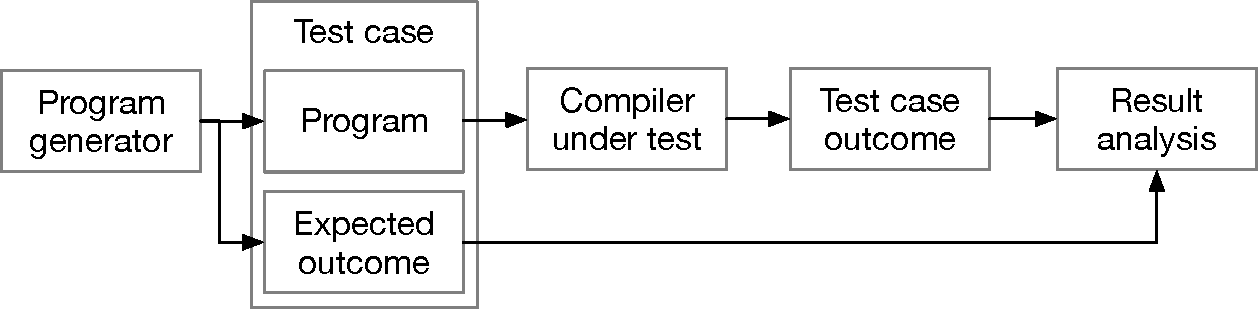
\includegraphics[width=.8\columnwidth]{img/oracle-generator}%
    \label{fig:test-case-generators-oracle}%
  }%
  \\*
  \subfloat[][Differential test case generation and evaluation]{%
    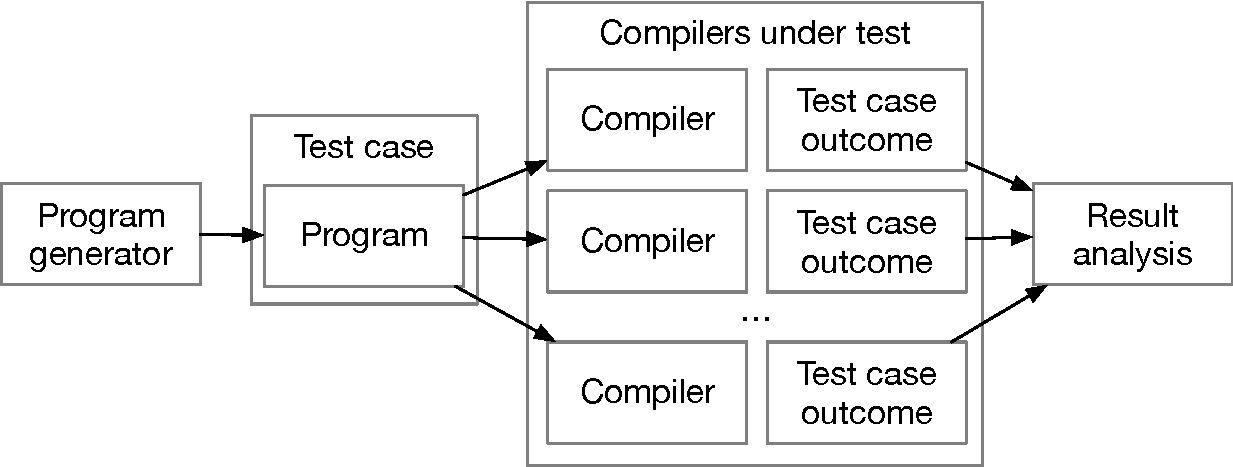
\includegraphics[width=.8\columnwidth]{img/difftest-generator}%
    \label{fig:test-case-generators-difftest}%
  }%
  \caption[Generating and evaluating compiler test cases]{%
    Two approaches to addressing the \emph{compiler validation} problem through test case generation. In~\protect\subref{fig:test-case-generators-oracle}, a test case comprises a program and its expected outcome. In~\protect\subref{fig:test-case-generators-difftest}, only a program is required, and the expected outcome is determined by majority voting on the observed outcomes across multiple compilers.%
  }%
  \label{fig:test-case-generators}
\end{figure}

Differential testing, illustrated in Figure~\ref{fig:test-case-generators-difftest}, accelerates testing by enabling multiple compilers to be tested at once. The idea is\ldots

\todo[inline]{Differential testing can be done across compilers, or using the same compiler with optimizations on or off (or a combination of the two). The two methodologies are empirically contrasted in~\cite{Chen2014a}, along with a comparison to Equivalemence Module Inputs (described in the next subsection).}

It is less sound than an oracle approach (since we don't have a golden standard for expected outcome), but in practise no work in the literature has reported false positives as a result. False negatives are unlikely, but not detectable ofc.

The advantage of differential testing over prior approaches is that it does not require a ground truth for the expected behaviour of a conformant compiler. As such, any well formed program may be used as a test. Even malformed inputs may be used to identify anlomies in compilers' error handling logic.

% McKeeman, W. M. (1998). Differential Testing for Software. DTJ, 10(1).
In the foundational work on differential testing for compilers, McKeeman \emph{et al.\ }present generators capable of enumerating programs of a range of qualities, from random ASCII sequences to C model conforming programs~\cite{McKeeman1998}. Subsequent works have presented increasingly complex generators which improve in some metric of interest, generally expressiveness or probability of correctness.

% Yang, X., Chen, Y., Eide, E., & Regehr, J. (2011). Finding and Understanding Bugs in C Compilers. In PLDI. https://doi.org/10.1145/2345156.1993532
CSmith~\cite{Yang2011} is a widely known and effective generator which enumerates programs by pairing infrequently combined language features. In doing so, it produces correct programs with clearly defined behaviour but very unlikely functionality, increasing the chances of triggering a bug. Achieving this required extensive engineering work, most of it not portable across languages, and ignoring some language features.

\todo[inline]{Extending CSmith to OpenCL took 8 man-months and 8000 lines of code~\cite{Lidbury2015a}.}

% Nagai, E., Hashimoto, A., & Ishiura, N. (2013). Scaling up Size and Number of Expressions in Random Testing of Arithmetic Optimization of C Compilers. In SASIMI.
Subsequent generators influenced by CSmith, like Orange3~\cite{Nagai2013}, focus on features and bug types beyond the scope of CSmith, arithmetic bugs in the case of Orange3.

% Bastani, O., Sharma, R., Aiken, A., & Liang, P. (2017). Synthesizing Program Input Grammars. In PLDI. https://doi.org/10.1145/3062341.3062349
Glade~\cite{Bastani2017} derives a grammar from a corpus of example programs. The derived grammar is enumerated to produce new programs, though unlike in this work, no distribution is learned over the grammar; program enumeration is uniformly random.

Programs generated by grammar-based approaches are often unlike real handwritten code, and are typically very large. As such, once a bug has been identified, test case reduction~\cite{Regehr2012a} is required to minimise the size of the program and isolate the code of interest.

One alternate method is to instead mutate a seed input, described below.


\subsubsection{Mutation and Feedback-directed Testing}


Equivalence Modulo Inputs (EMI) testing~\cite{Le2013a,Sun2016a} follows a different approach to test case generation. Starting with existing code, it inserts or deletes statements that will not be executed, so functionality should remain the same. If it is affected, it is due to a compiler bug. While a powerful technique able to find hard to detect bugs, it relies on having a very large number of programs to mutate. As such, it still requires an external code generator. Similarly to CSmith, EMI favours very long test programs.

LangFuzz~\cite{Holler2012} also uses mutation but does this by inserting code segments which have previously exposed bugs. This increases the chances of discovering vulnerabilities in scripting language engines.

Skeletal program enumeration~\cite{Zhang2017a} again works by transforming existing code. It identifies algorithmic patterns in short pieces of code and enumerates all the possible permutations of variable usage.

A mutation-based approach for differential testing the Java Virtual Machine is demonstrated in~\cite{Chena}.

% Cheng, L., Zhang, Y., Zhang, Y., Wu, C., Li, Z., Fu, Y., & Li, H. (2019). Optimizing seed inputs in fuzzing with machine learning. ArXiv:1902.02538.
\todo[inline]{Neural networks are used to discover correlation between PDF test case and execution in the target program. The correlations are then leveraged to generate new paths in the target program~\cite{Cheng2019}.}

% Wang, J., Chen, B., Wei, L., & Liu, Y. (2017). Skyfire: Data-Driven Seed Generation for Fuzzing. In S&P. https://doi.org/10.1109/SP.2017.23
Skyfire~\cite{Wang2017c} learns a probabilistic context-sensitive grammar over a corpus of programs to generate input seeds for mutation testing. The generated seeds are shown to improve the code coverage of AFL~\cite{Zalewski} when fuzzing XSLT and XML engines, though the seeds are not directly used as test cases.

% Mathis, B., Kampmann, A., Gopinath, R., Höschele, M., Mera, M., & Zeller, A. (2019). Parser-Directed Fuzzing. In PLDI.
\todo[inline]{PLDI'19 fuzzing paper~\cite{Mathis2019}.}

% Peng, H., Shoshitaishvili, Y., & Payer, M. (2018). T-Fuzz: Fuzzing by Program Transformation. In SP.
\todo[inline]{Starting with a coverage-guided set of inputs, \emph{T-Fuzz} uses dynamic tracing to detect input checks in programs, and removes them~\cite{Peng2018}.}


\subsubsection{Neural Program Generation}

% Sutskever, I., Vinyals, O., & Le, Q. V. (2014). Sequence to Sequence Learning with Neural Networks. In NIPS.
\todo[inline]{Many methods based on sequence-to-sequence learning~\cite{Sutskever2014}.}

RNNs have been successfully applied to a variety of other generative tasks, including image captioning~\cite{Vinyals}, colourising black and white photographs~\cite{Zhang2016}, artistic style~\cite{Gatys2015}, and image generation~\cite{Gregor2014}.

The proficiency of LSTMs for sequence modelling is demonstrated in~\cite{Sutskever2014}. \citeauthor{Sutskever2014} apply two LSTM networks to translate first a sequence into a fixed length vector, then to decode the vector into an output sequence. This architecture achieves state-of-the-art performance in machine translation. The authors find that reversing the order of the input sequences markedly improves translation performance by introducing new short term dependencies between input and output sequences.

The application of language modelling for generating executable programs is novel. In training on large corpuses of hand-written code, the language model learns the human biases which are present in common codes~\cite{Caliskan-islam2016}. While such human-induced biases can prove controversial in social domains~\cite{Bolukbasi2016,Joseph2017}, this enables the generation of programs which, unlike other approaches to program generation, are representative of real workloads.

% White, M., Vendome, C., Linares-Vasquez, M., & Poshyvanyk, D. (2015). Toward Deep Learning Software Repositories. In MSR.
\todo[inline]{Deep learning over code has long been a goal of research~\cite{White2015a}.}

% Jozefowicz, R., Vinyals, O., Schuster, M., Shazeer, N., & Wu, Y. (2016). Exploring the Limits of Language Modeling. arXiv:1602.02410.
\todo[inline]{Limits of language modelling~\cite{Jozefowicz2016a}.}

% Neelakantan, A., Le, Q. V., & Sutskever, I. (2016). Neural Programmer: Inducing Latent Programs with Gradient Descent. In ICLR.
\todo[inline]{Early program generation from latent variables~\cite{Neelakantan2016}.}

% Godefroid, P., Peleg, H., & Singh, R. (2017). Learn&Fuzz: Machine Learning for Input Fuzzing. In ASE.
Most similar to this work is Learn\&fuzz~\cite{Godefroid2017}, in which an LSTM network is trained over a corpus of PDF files to generate test inputs for the Microsoft Edge renderer, yielding one bug. Unlike compiler testing, PDF test cases require no inputs and no pre-processing of the training corpus.

% Brockschmidt, M., Allamanis, M., Gaunt, A. L., & Polozov, O. (2018). Generative Code Modeling with Graphs. Retrieved from http://arxiv.org/abs/1805.08490
\citeauthor{Brockschmidt2018} present a novel methodology for program generation in which a graph is used as the intermediate representation~\cite{Brockschmidt2018}. While the generated

% Liu, X., Li, X., Prajapati, R., & Wu, D. (2019). DeepFuzz: Automatic Generation of Syntax Valid C Programs for Fuzz Testing. In AAAI.
\todo[inline]{\emph{DeepFuzz} uses a sequence-to-sequence model to generate C programs. Found 8 bugs in GCC. Unlike this work: all whitespace is replaced with a single space. Sampling only occurs on whitespace, this maximises probabilty of syntactic correctness, but not semantic~\cite{Liu2019}.}

% Nasrabadi, M. Z., Parsa, S., & Kalaee, A. (2018). Neural Fuzzing: A Neural Approach to Generate Test Data for File Format Fuzzing. ArXiv:1812.09961. Retrieved from https://arxiv.org/pdf/1812.09961.pdf
\todo[inline]{\emph{IUST DeepFuzz} is a file neural generator for file format fuzzing, tested on PDFs~\cite{Nasrabadi}.}

% She, D., Pei, K., Epstein, D., Yang, J., Ray, B., & Jana, S. (2018). NEUZZ: Efficient Fuzzing with Neural Program Learning. ArXiv:1807.05620.
\todo[inline]{\emph{NEUZZ} learns a differentiable neural approximation of target program logic, use SGD to guide mutation. I like this idea! Using ML to \emph{guide} program generation removes the worry of ML system having to correctly learn PL semantics. This doesn't simplify the approach though~\cite{She2018}.}

Machine learning has been used for other purposes in testing other than program generation. These are reviewed in Section~\ref{sec:related-work-other}.
